\section{Discussion of results}
\hyperlink{function2_plot}{Code for generating plots}\\
As we can see error for 'B' system of equations increased after our residual correction. But that's just one matrix and vector pair, after testing more pairs we get following graphs (Tested on systems of equations from a) and b) respectively, with maximum size of matrices and vectors equal to 100):
\begin{center}
   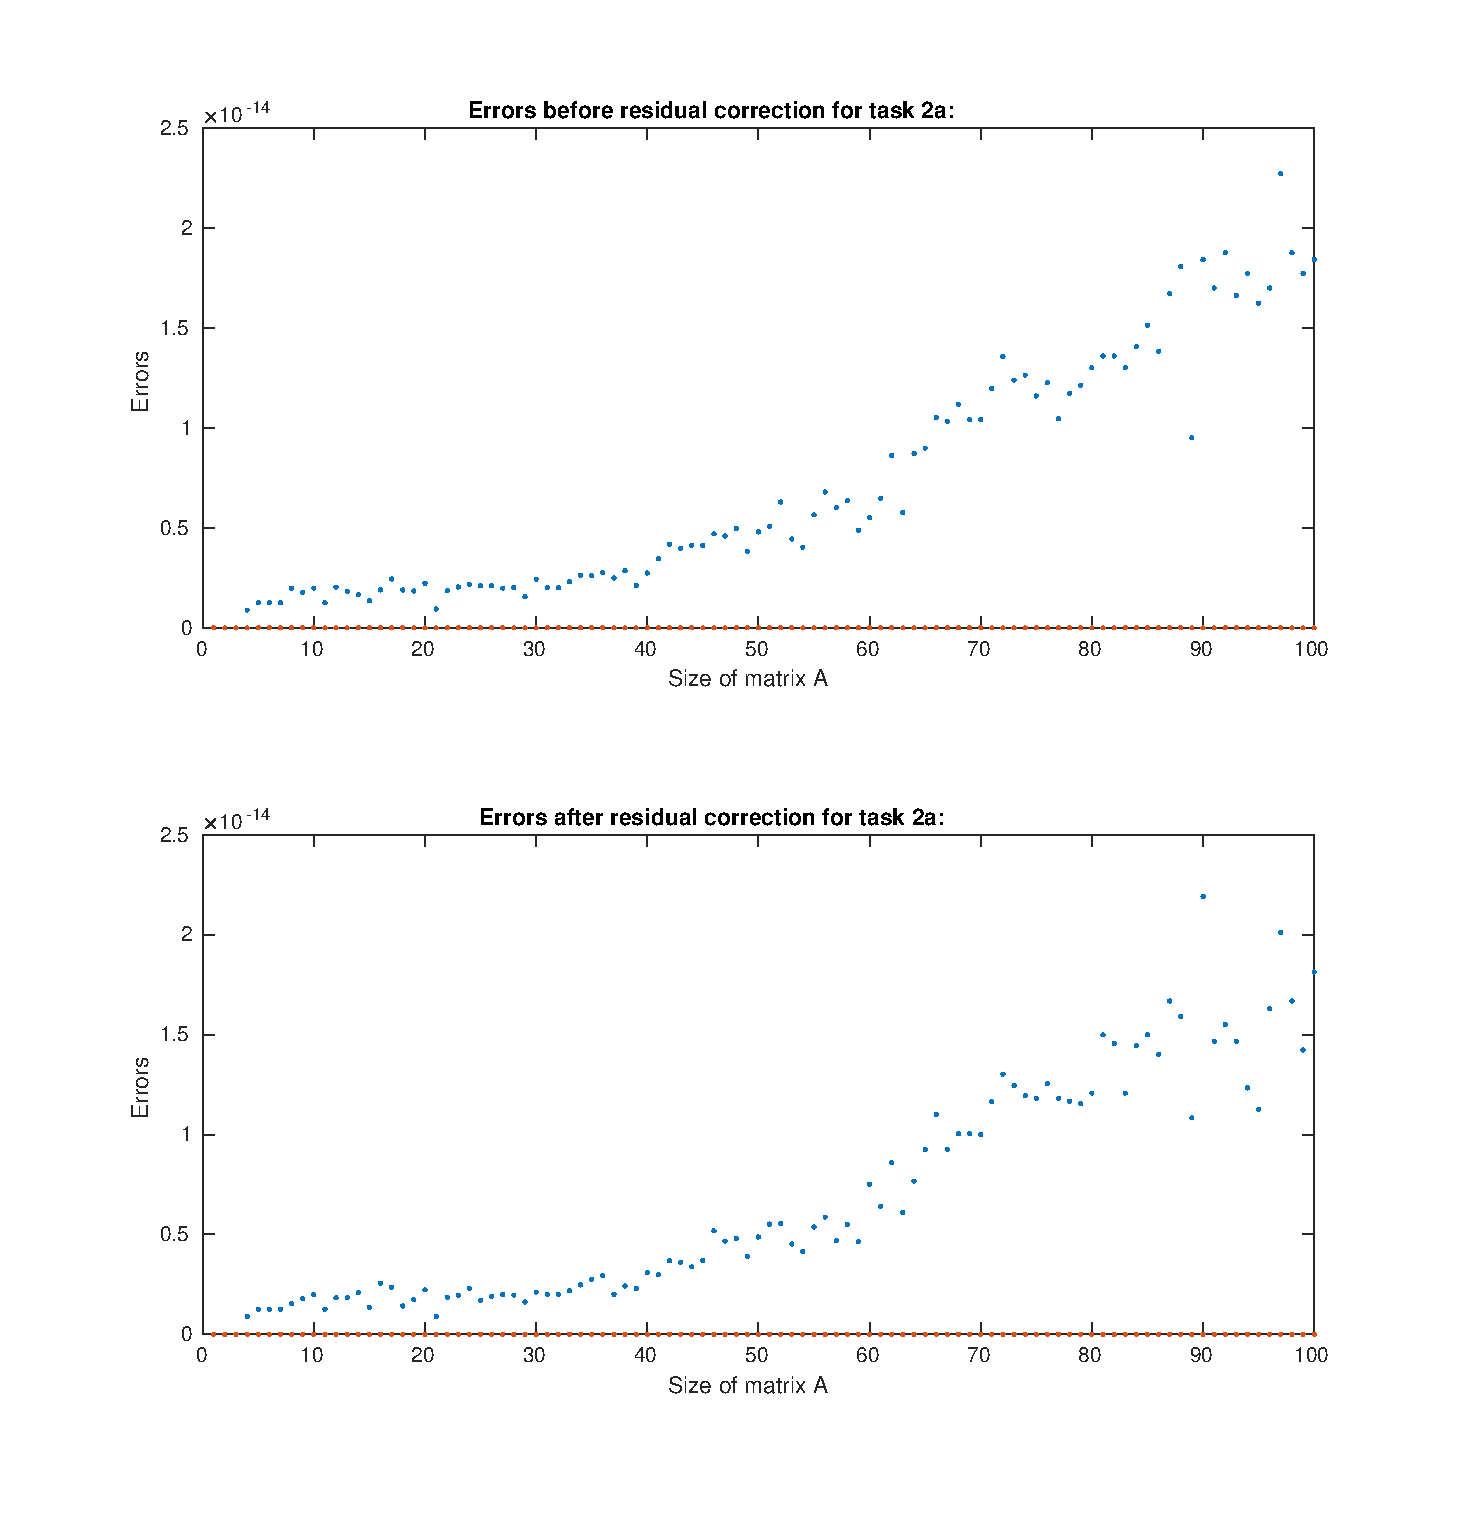
\includegraphics[scale=0.5]{errorsA.eps}
\end{center}

\begin{center}
   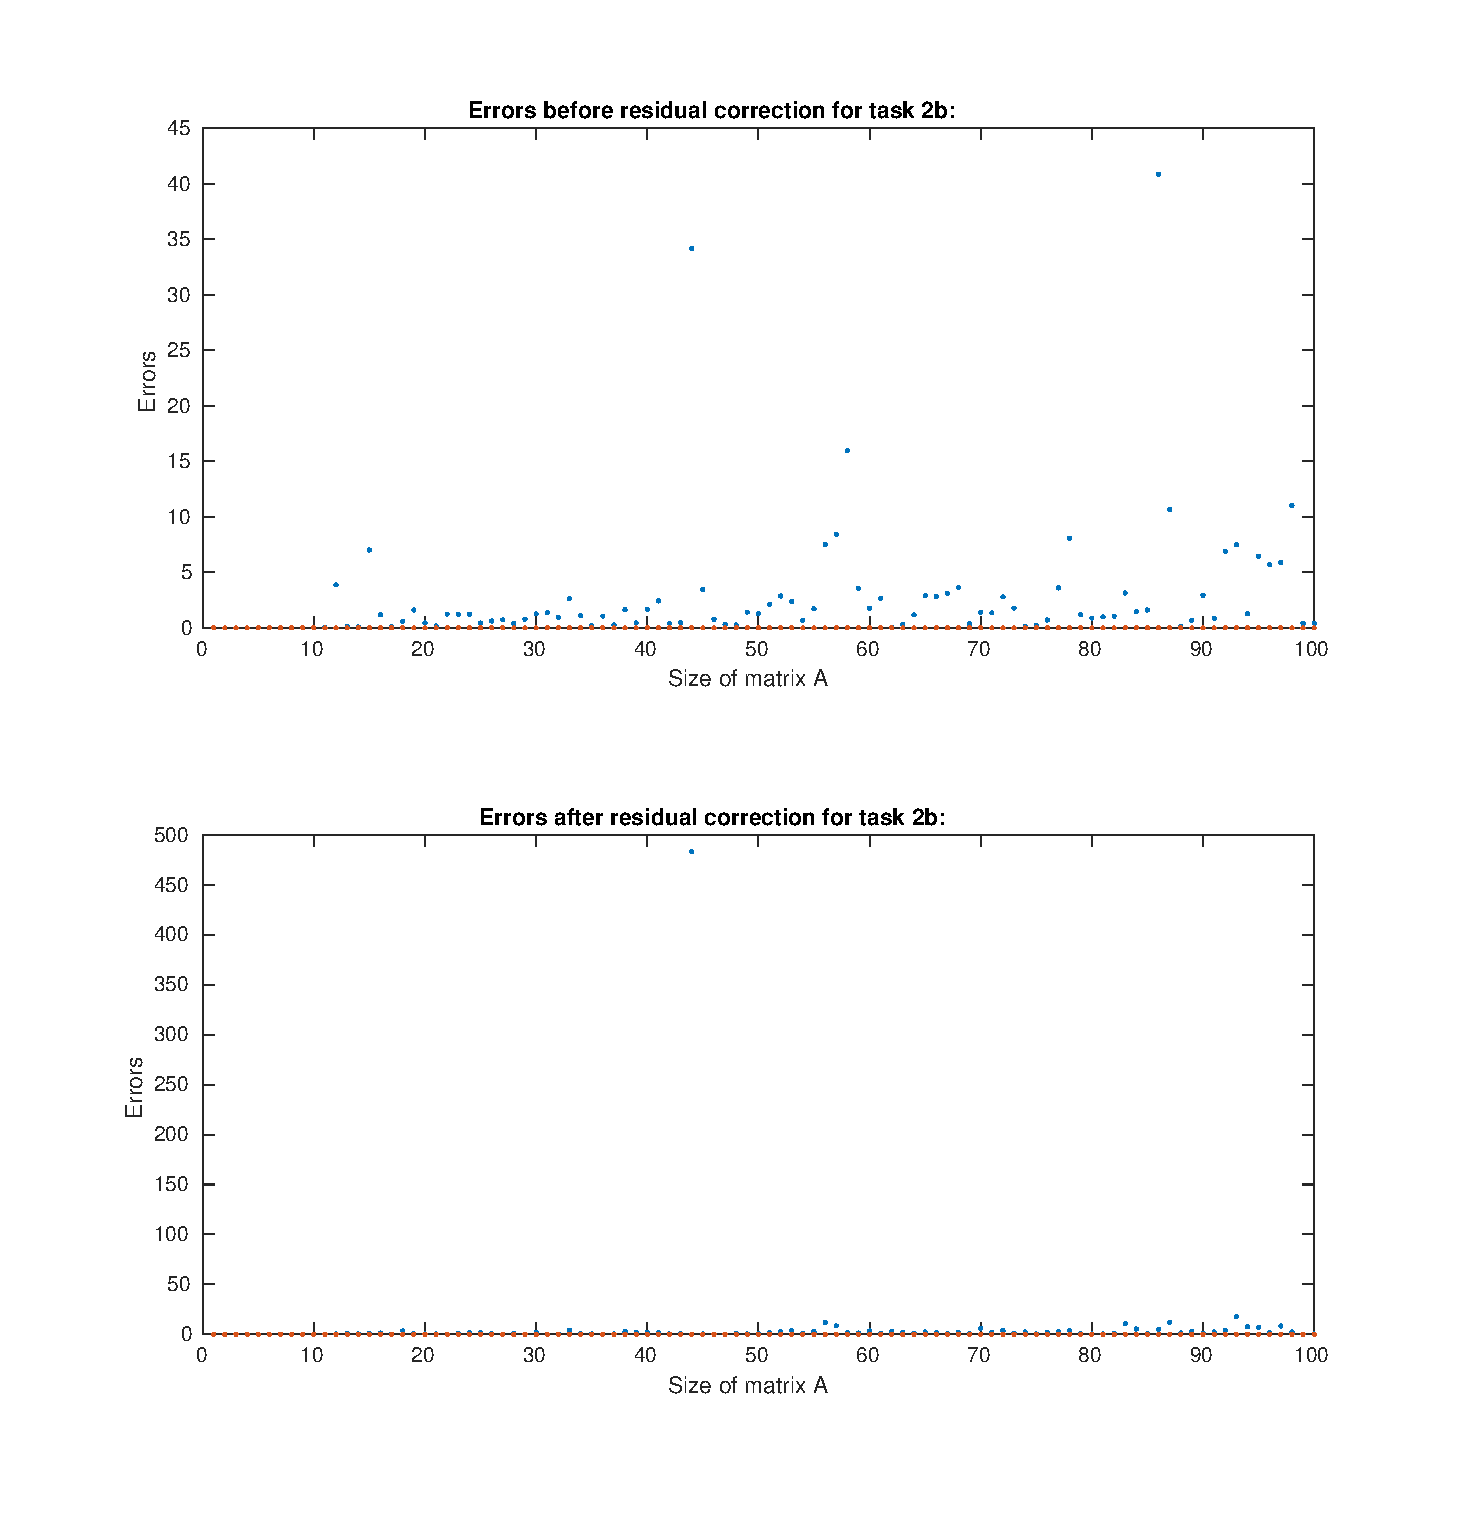
\includegraphics[scale=0.5]{errorsB.eps}
\end{center}
As we can see our residual correction method \textbf{does} work for Matrix B and Vector B and decreases the error drastically.

\subsection{Errors in b)}
Matrix B suffers from relatively huge errors. Where do they come from?
Matrix B is a variant of Hilbert matrix.
Equation for generating elements of this matrix is as follows:
\[ b_{ij} = \frac{5}{8(i + j + 1)} \]
Equation for generating elements of the Hilbert matrix is as follows:
\[ b_{ij} = \frac{1}{(i + j - 1)} \]
The only thing that changes are the constants, we have 5 instead of 1 in the numerator and 8 in front of the summation in the denominator and +1 instead of -1. For sufficiently huge 'i' and 'j' those differences hardly matter.
Hilbert matrix is badly conditioned. It's condtion number for \textit{n} size hilbert matrix is equal to:
\[ \mathcal{O}(\frac{e^{3.5255n}}{sqrt(n)}) \]
Let's calculate condition number of matrix B in matlab:
\begin{simplechar}
\begin{lstlisting}
cond(matrixB(10))
ans = 2.428027097978043e+14
\end{lstlisting}
\end{simplechar}

And compare it with condition number of matrix A:
\begin{simplechar}
\begin{lstlisting}
cond(matrixA(10))
ans = 4.550344127923193
\end{lstlisting}
\end{simplechar}
As we can see the difference is huge, conditon number of matrix B for 10 elements is $10^{14}$ times bigger than for matrix A. This explains big errors for matrix B.











\addtocontents{toc}{\protect\newpage}
\chapter{Problem 3 - Solving a system of n linear equations - iterative algorithm}

